\section{Kailath 4.1-8}
The model:
\begin{align*}
    \ddot x - 2\omega\dot y - 9\omega^2x &= 0 & \ddot y + 2\omega\dot x + 4\omega^2y &= u.
\end{align*}
Let, 
\begin{align*}
    \dot x &= v_x, \quad \dot y = v_y & \implies \ddot x = \dot v_x, \quad \ddot y &= \dot v_y. 
\end{align*}
Therefore, 
\begin{align*}
    \dot v_x - 2\omega v_y - 9\omega^2x &= 0 & \dot v_y + 2\omega v_x + 4\omega^2y &= u, \\
    \dot v_x &= 2\omega v_y + 9\omega^2x & \dot v_y &= u - 2\omega v_x - 4\omega^2y. \\
\end{align*}
The state matrix, $X = \begin{pmatrix} x & v_x & y & v_y \end{pmatrix}^T$. The system can be re-written as 
\newcommand{\A}{\begin{pmatrix}
    0 & 1 & 0 & 0\\
    9\omega^2 & 0 & 0 & 2\omega \\
    0 & 0 & 0 & 1 \\
    0 & -2\omega & -4\omega^2 & 0 
\end{pmatrix}}
\begin{align*}
    \dot X &= \A\,X + \begin{pmatrix}
        0 \\ 0 \\ 0 \\ 1
    \end{pmatrix}\,u, & y &= \begin{pmatrix}
        0 & 0 & 1 & 0
    \end{pmatrix}\,X.
\end{align*}
The closed-loop observer poles 
\begin{align*}
    \alpha_\mathcal{O}(s) &= \text{det}\left(SI - A + K\,C\right) \\
    &= \text{det}\left(\begin{pmatrix}
        s & 0 & 0 & 0 \\ 0 & s & 0 & 0 \\ 0 & 0 & s & 0 \\ 0 & 0 & 0 & s
    \end{pmatrix} - \A + \begin{pmatrix}
        k_1 \\ k_2 \\ k_3 \\ k_4
    \end{pmatrix}\,\begin{pmatrix}
        0 & 0 & 1 & 0
    \end{pmatrix}\right) \\
    &= \text{det}\begin{pmatrix}
        s & -1 & k_1 & 0 \\ -9\omega^2 & s & k_2 & -2\omega \\ 0 & 0 & k_3 + s & -1 \\ 0 & 2\omega & 4\omega^2 + k_4 & s
    \end{pmatrix}\\
    &= s^4 + k_3s^3 + \left(k_4 - \omega^2\right)s^2 + (-5k_3\omega^2-2k_2\omega)s - 36\omega^4 - 18k_1\omega^3 - 9k_4\omega^2
\end{align*}
The closed-loop observer poles are $s = -2\omega$, $s = -3\omega$, $s = -3\omega \pm j3\omega$
\begin{align*}
    \alpha_\mathcal{O}(s) &= \left(s + 2\omega\right)\,\left(s + 3\omega_0\right)\,\left(s + 3\omega - j3\omega\right)\,\left(s + 3\omega + j3\omega\right) \\
    &= s^4 + 11\omega s^3 + 54\omega^2 s^2 + 126\omega^3 s + 108\omega^4
\end{align*}
Now, 
\begin{align*}
    \begin{array}{rcl}
        k_3 & = & 11\omega \\
        k_4 - \omega^2 & = & 54\omega^2 \\
        5k_3\omega^2 + 2k_2\omega & = & -126\omega^3 \\
        36\omega^4 + 18k_1\omega^3 + 9k_4\omega^2 & = & -108\omega^4
    \end{array} \qquad \implies \begin{array}{rcl}
        k_1 & = & -\frac{71}{2}\omega \\ 
        k_2 & = & -\frac{181}{2}\omega^2 \\
        k_3 & = & 11\omega \\ 
        k_4 & = & 55\omega^2.
    \end{array} 
\end{align*}
The observer is 
\begin{align*}
    \dot{\hat X} &= A\,\hat X + B\,u + K\,\left(y - C\,\hat X\right)
\end{align*}
The simulation results are shown in the figure below, the blue curve is the 'true' state and rthe orange is the estimated from the observer.

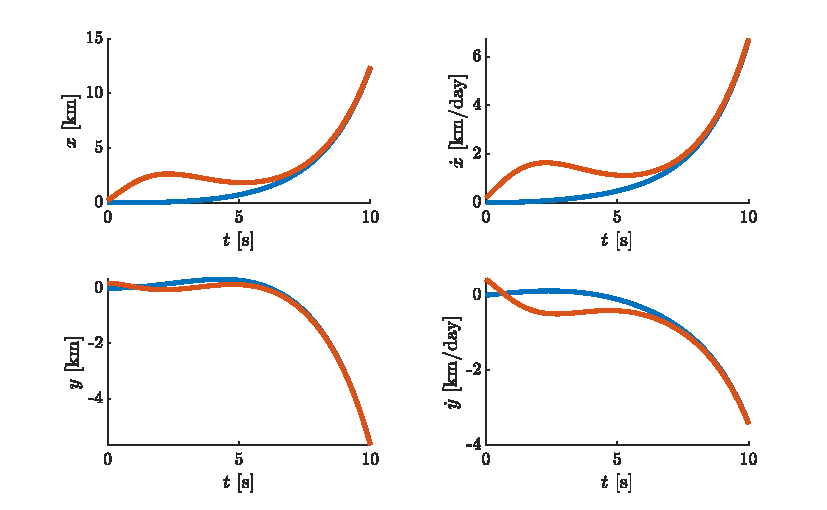
\includegraphics{figures/ex418.pdf}

The error between the estimated states and the 'true' states is shown 

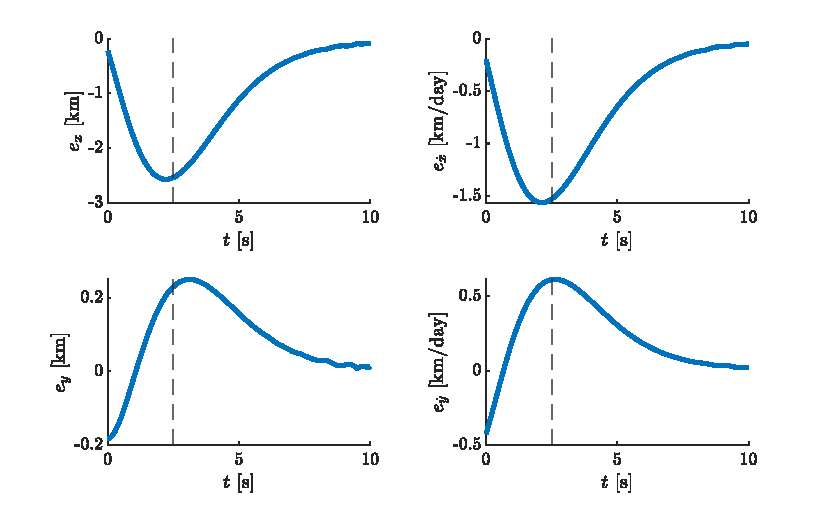
\includegraphics{figures/ex418_err.pdf}

From the figure, it is clear that after 2.5\,days the error starts to decay.

\subsection*{Code}
\matlabheading{Algebra}

\begin{matlabcode}
syms s w
e1 = collect((s + 2*w) * (s + 3*w) * ... 
        ... (s + 3*w + 1j*3*w) * (s + 3*w - 1j*3*w),s);
c1 = coeffs(e1,s); c1(end) = [];
S = s*eye(4);
A = [0, 1, 0, 0;...
     9*w^2, 0, 0, 2*w;...
     0, 0, 0, 1;...
     0, -2*w, -4*w^2, 0]; 
K = sym('k',[4 1]); C = [0 0 1 0];
e2 = collect(det(S - A + K*C),s);
c2 = coeffs(e2,s); c2(end) = [];
eqns = c1 == c2; 
Sol = solve(eqns,K); 
\end{matlabcode}

\matlabheading{system simulation (true-states)}

\begin{matlabcode}
omega = 2*pi/29.3; % orbital frequency [rad/s]
u = 1000 / (300 * omega^2) ; % input (F/(m*w^2)) [m/rad^2]
% state space representation [x; xdot; y; ydot]
A = [0, 1, 0, 0;...
     9*omega^2, 0, 0, 2*omega;...
     0, 0, 0, 1;...
     0, -2*omega, -4*omega^2, 0];
B = [0; 0; 0; 1]; C = [0, 0, 1, 0];
bryson_sattelite = @(t,x) A*x + B*u;

% simulation
y0 = [0; 0; 0; 0]; % initial states
tspan = [0 10]; % [days]
[t, y] = ode45(@(t,y) bryson_sattelite(t,y),tspan,y0);
\end{matlabcode}

\matlabheading{observer}

\begin{matlabcode}
% state observer 
K = [-71/2*omega; -181/2*omega^2; 11*omega; 55*omega^2];
mesh = @(x) interp1(t,y(:,3),x);
obs_bryson_sattelite = @(t,x) A*x + B*u + K*(mesh(t) - C*x);

% simulation 
y0 = rand([4 1]) * 500; % initial states
[to, yo] = ode45(@(t,y) obs_bryson_sattelite(t,y),tspan,y0); 

% error
for ii = 1:width(y)
    yq = interp1(t,y(:,ii),to);
    eq(:,ii) = yq - yo(:,ii);
end
\end{matlabcode}